\documentclass{article}
\makeatletter
\renewcommand{\fnum@figure}{Εικόνα \thefigure}
\makeatother
\usepackage[greek, english]{babel}
\usepackage{alphabeta}
\usepackage{atbegshi, picture}
\usepackage[letterpaper,top=2cm,bottom=2cm,left=3cm,right=3cm,marginparwidth=1.75cm]{geometry}
\usepackage{amsmath}
\usepackage{graphicx}
\usepackage[colorlinks=true, allcolors=blue]{hyperref}
\usepackage[utf8]{inputenc}
\usepackage{indentfirst}
\usepackage[table]{xcolor}

\addto\captionsenglish{
  \renewcommand{\contentsname}
    {Περιεχόμενα}
}

\newcommand\T{\rule{0pt}{2.6ex}}       % Top strut
\newcommand\B{\rule[-1.2ex]{0pt}{0pt}} 

\begin{document}



\begin{titlepage}
   \begin{center}
       \vspace*{1cm}

       \textbf{\huge Risk Assessment}

       \vspace{0.5cm}
        Τεχνολογία Λογισμικού
            
       \vspace{1cm}

       \textbf{Βεργίνης Δημήτριος\\Βλαχογιάννης Δημήτριος}
       
       \begin{figure}[!htb]
        \centering
        
\includegraphics[width=0.5\textwidth]{logo.png}
        \end{figure}
        
        \vspace{0.5cm}
        
        \begin{figure}[!htb]
        \centering
        
\includegraphics[width=0.5\textwidth]{ceid.jpg}
        \end{figure}


       \vfill
            
       Τεχνικό Κείμενο για την Τεχνολογία Λογισμικού\\
            
       \vspace{0.5cm}
            
       CEID, ECE\\
       University of Patras\\
            
   \end{center}
\end{titlepage}

\noindent Η ομάδα μας

\begin{enumerate}
  \item Βεργίνης Δημήτριος, ΑΜ: 10166634 , ECE
  \item Βλαχογιάννης Δημήτριος, ΑΜ: 1067371, CEID
  \item Κούρου Αγγελική, ΑΜ: 1067499 , CEID
  \item Μητροπούλου Αικατερίνα - Quality Manager, ΑΜ: 1067409, CEID
  \item Στεφανίδης Μάριος - Project Manager, ΑΜ:1067458, CEID
\end{enumerate}
{
  \hypersetup{linkcolor=black}
  \tableofcontents
}

\section{Περιγραφή}
Στο παρακάτω κείμενο θα γίνει μια αρχική παρουσίαση των κλάσεων που θα απαρτίζουν τον σχεδιασμό του \textbf{Medic World}. 

\vspace{1cm}

\section{Domain Diagram}
Παρακάτω φαίνεται το αρχικό σχήμα του domain model. Για περαιτέρω βοήθεια στην κατανόηση πρέπει
να γίνουν οι εξής διευκρινίσεις:

\begin{itemize}
    \item Με απλή γραμμή συμβολίζουμε την απλή συσχέτιση μεταξύ των κλάσεων.
    \item Η διακεκομμένη γραμμή δηλώνει χαλαρές συσχετίσεις ανάμεσα στις κλάσεις.
    \item Με το τρίγωνο παρουσιάζουμε τις σχέσεις κληρονομικότητας.
    \item Η γραμμή με τον άδειο ρόμβο αναπαριστά την σχέση συνάθροισης.
    \item Ο μαύρος ρόμβος συμβολίζει σχέσεις σύνθεσης.
\end{itemize}


\begin{figure}[!htb]
        \centering
        \includegraphics[width=0.5\textwidth]{arrows.png}
        \end{figure}


\begin{figure}[!htb]
        \centering
        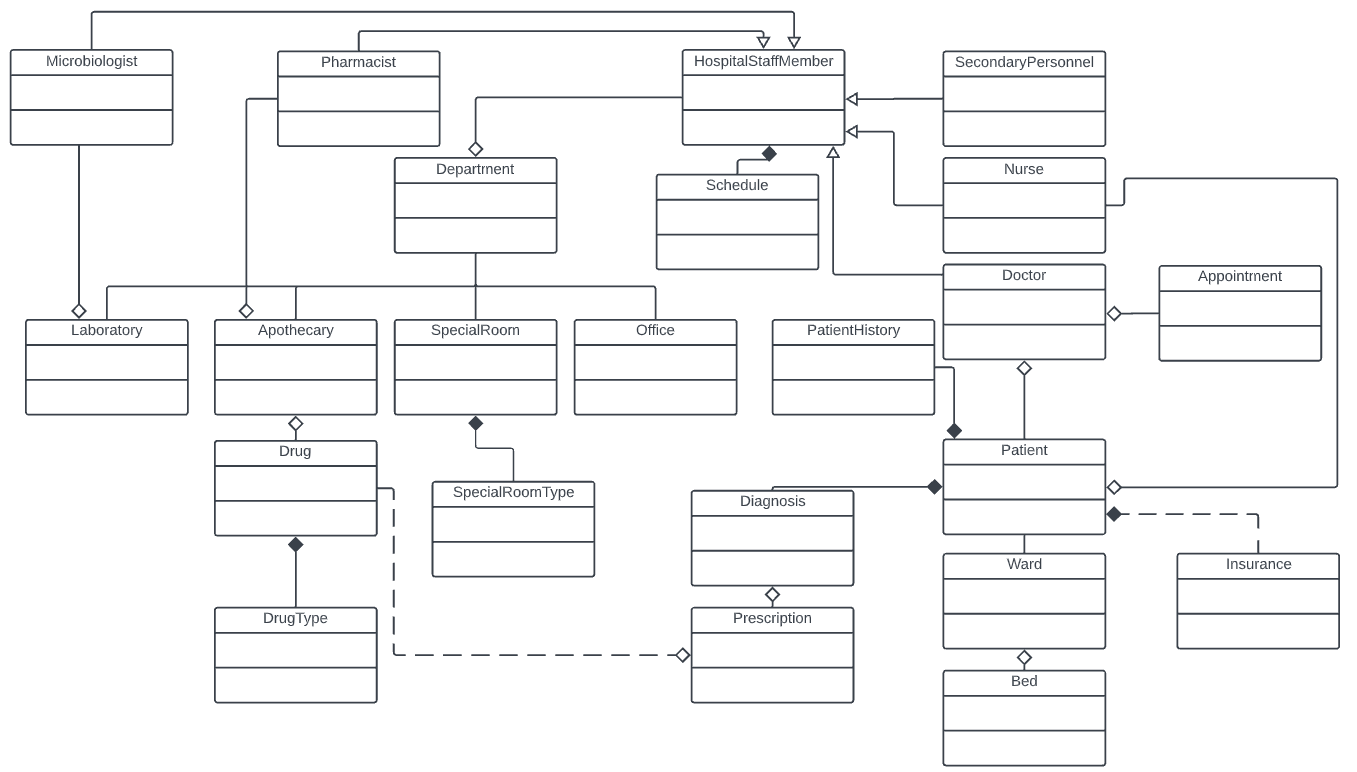
\includegraphics[width=1.0\textwidth]{domain.png}
        \end{figure}

\section{Ανάλυση κλάσεων}

\begin{itemize}
    \item \textbf{HospitalStaffMemeber}: Είναι η βασική οντότητα που περιέχει όλο το προσωπικό του νοσοκομείου, περιλαμβάνει ιδιότητες μοναδικές για κάθε άτομο (π.χ. ονοματεπώνυμο, αφμ, μισθος κ.α.).
    \item \textbf{Pharmacist}: Ειδικότερη κατηγορία υπαλλήλου του νοσοκομείου. Υπεύθυνος διαχείρησης της οντότητας Apothecary (φαρμακείου).
    \item \textbf{Department}: Οντότητα που αναπαριστά τα διάφορα τμήματα του νοσοκομείου (π.χ. Ενδοκρινολογικό, Ακτινολογικό).
    \item \textbf{Apothecary}: Συστατικό μέρος του τμήματος, περιλαμβάνει όλα τα απαραίτητα για την εύρυθμη λειτουργία της υπηρεσίας, φάρμακα.
    \item \textbf{Drug}: Οντότητα που περιέχει τις γενικές πληροφορίες για το κάθε φάρμακο (ημ.παραλαβης, απόθεμα) καθώς και σε ποιον ασθενή έχει συνταγογραφηθεί.
    \item \textbf{DrugType}: Κλάση που περιέχει το είδος του κάθε φαρμάκου και τη χρήση που αυτό θα έχει (αντιφλεγμονώδες, αντιπυρετικό κ.α).
    \item \textbf{SpecialRoom}: Αποτελεί το κάθε ειδικό δωμάτιο μέσα στο νοσοκομείο το οποίο δεν είναι κάποια απλή κλίνη και δηλώνει το αν αυτό είναι διαθέσιμο για χρήση.
    \item \textbf{RoomType}:Καθορίζει το είδος του ειδικού δωματιού το οποίο μπορεί αν είναι χειρουργείο, δωμάτιο μαγνητικού τομογράφου κ.α..
    \item \textbf{Office}: Οντότητα που αναπαριστά το γραφείου του προσωπικού.
    \item \textbf{Schedule}: Αποκλειστικό πρόγραμμα για κάθε ένα από τους υπαλλήλους, το οποίο δεν είναι σταθερό.
    \item \textbf{Doctor}: Ειδίκευση της οντότητας του προσωπικού, συσχετίζεται με τους ασθενείς.
    \item \textbf{Patient}: Κλάση που περιέχει όλες τις βασικές πληροφοριές για τον ασθενή.
    \item \textbf{PatientHistory}: Ειδική οντότητα που περιλαμβάνει το ιστορικό του ασθενή (παλαιότερες επισκέψεις, ασθένειες, κληρονομικότητα).
    \item \textbf{Diagnosis}: Η διάγνωση του ασθενή που προκύπτει από την εκάστοτε επίσκεψη του ασθενούς στο νοσοκομείο και την εξέταση από το γιατρό.
    \item \textbf{Prescription}: Η συταγογράφηση του γιατρού προς τον ασθενή εφόσον αυτή κριθεί απαραίτητη από την εξέταση.
    \item \textbf{Ward}: Οντότητα που αναπαριστά την πτέρυγα του νοσοκομείου στην οποία βρίσκεται ο ασθενής εφόσον έχει εισαχθεί.
    \item \textbf{Bed}: Η ακριβής κλίνη στην οποία βρίσκεται ο ασθενής.
    \item \textbf{Insurance}: Κλάση που περιέχει τις λεπτομέρειες για την ασφάλεια που κατέχει ο ασθενής για την κάλυψη των ιατρικών του εξόδων.
    \item \textbf{Appointment}: Οντότητα που περιλαμβάνει τις πληροφορίες για τα ραντεβού του ιατρού και τις λοιπές κλινικές του υποχρεώσεις.
    \item \textbf{Nurse}: Ειδίκευση της οντότητας του προσωπικού, μια νοσοκόμα μπορεία να είναι υπεύθυνη για παραπάνω από έναν ασθενή.
    \item \textbf{SecondaryPersonnel}: Το λοιπό προσωπικό του νοσοκομείου, περιλαμβάνει όλο το τεχνικό προσωπικό, μέλη της διοίκησης κ.α.
\end{itemize}


\end{document}